\documentclass{article}
\usepackage{graphicx} 

\title{Problem Set 6}
\author{Steven Plaisance}
\date{March 2023}

\begin{document}

\maketitle

I chose to use the NFL Draft data that I pulled from the collegefootballdata.com API via the R package cfbfastR (in Problem Set 5) for this problem set. I will outline the steps I took below.

\begin{enumerate}
  \item Because the function to download draft picks requires a specified year, I created a simple for loop to compile all data from 2000 to 2022 into a single data frame.
  \item In terms of data cleaning/transformation, my primary goal was to create a draft capital metric to measure how much draft capital teams were allocating to various positions. I created a simple version by inverting the overall draft position value. The first overall pick takes on a value of ~250, while the last pick takes on a value of 1, etc. 
  \item I then grouped the data by year and position and calculated two key variables: total capital and average capital. Total capital represents the total draft capital allocated to each position, while average capital represents the average capital aqllocated to each player drafted at that position. 
  \newpage
  \item My first visualization looks at a position that has largely faded into irrelevance, the fullback. These powerful blockers have become less valuable with the rise of passing in the NFL and the expanded skill-set of the modern tight end. Our visualization corroborates this theme.
  
  \linebreak
  \linebreak
      \parbox{\linewidth}{
        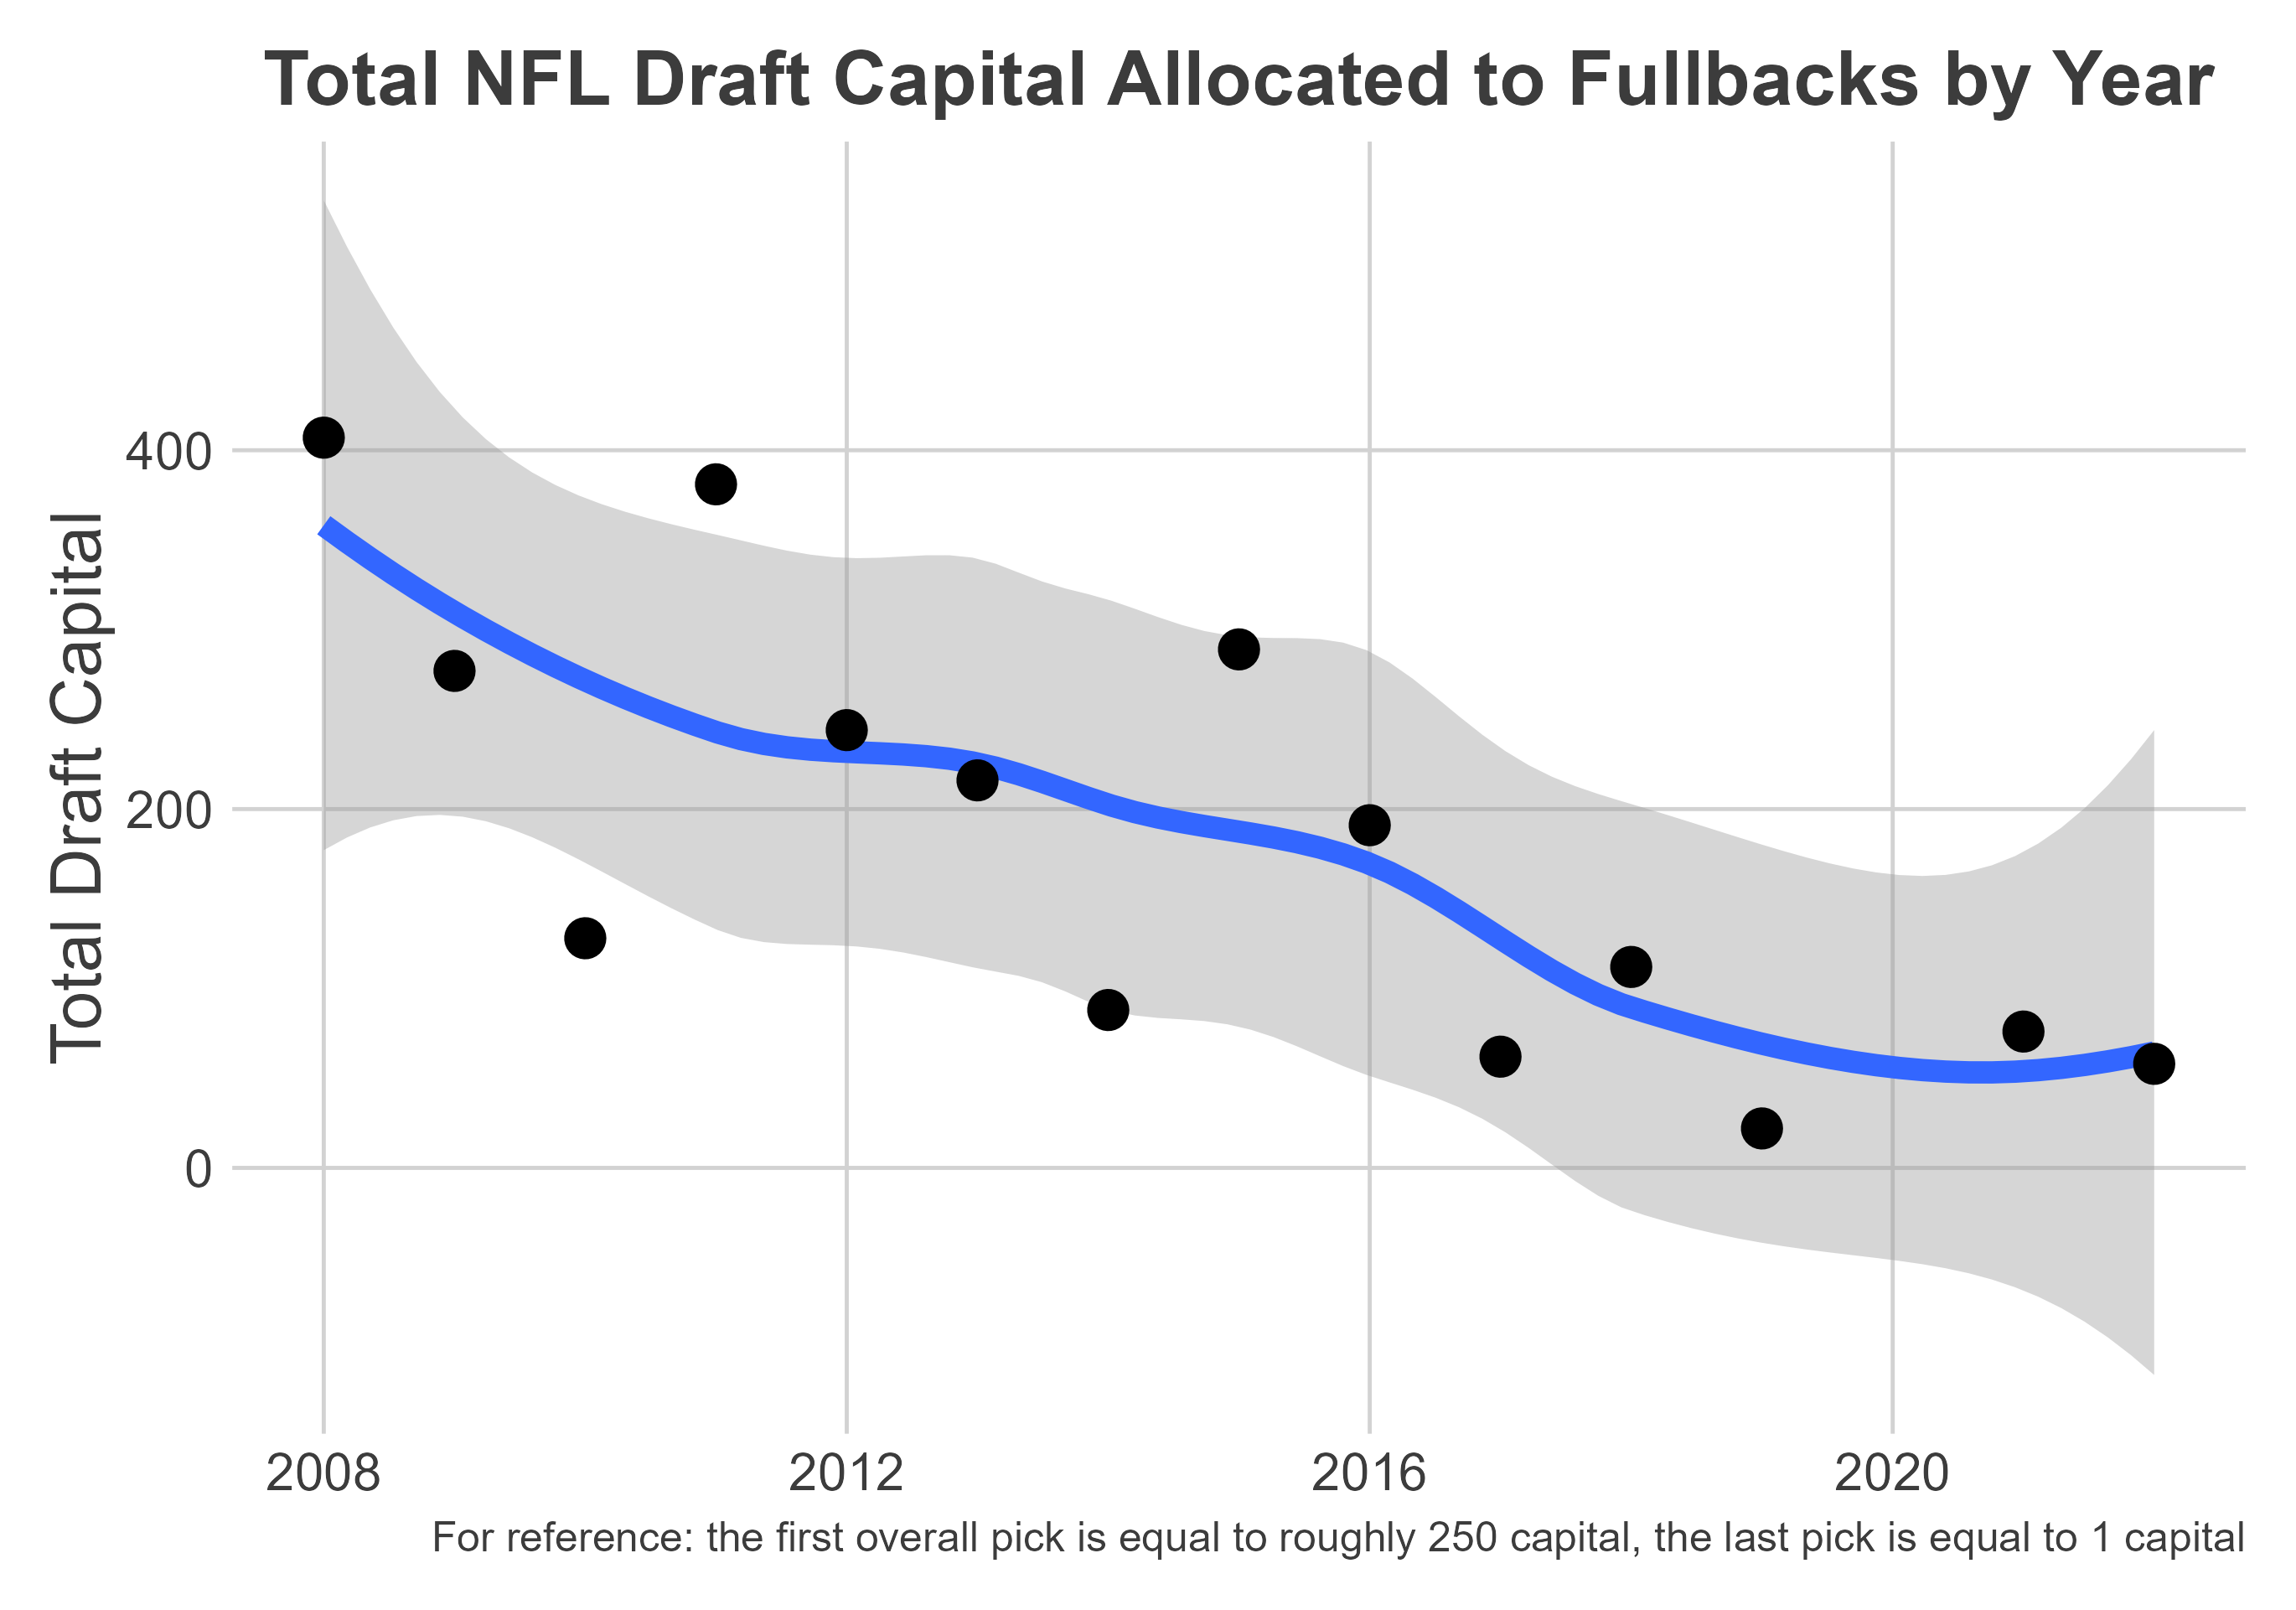
\includegraphics[width=14cm]{PS6a_Plaisance.png}
        \centering
        \\}
  \newpage
  \item Next we'll turn to the most valuable position in sports: the quarterback. As passing has increased in the NFL, teams have begun to place even greater value on the QB. Because teams still only roster 2 quarterbacks, the total capital allocated has not changed much. But the average capital has increased, as seen here.
  
    \linebreak
    \linebreak
      \parbox{\linewidth}{
        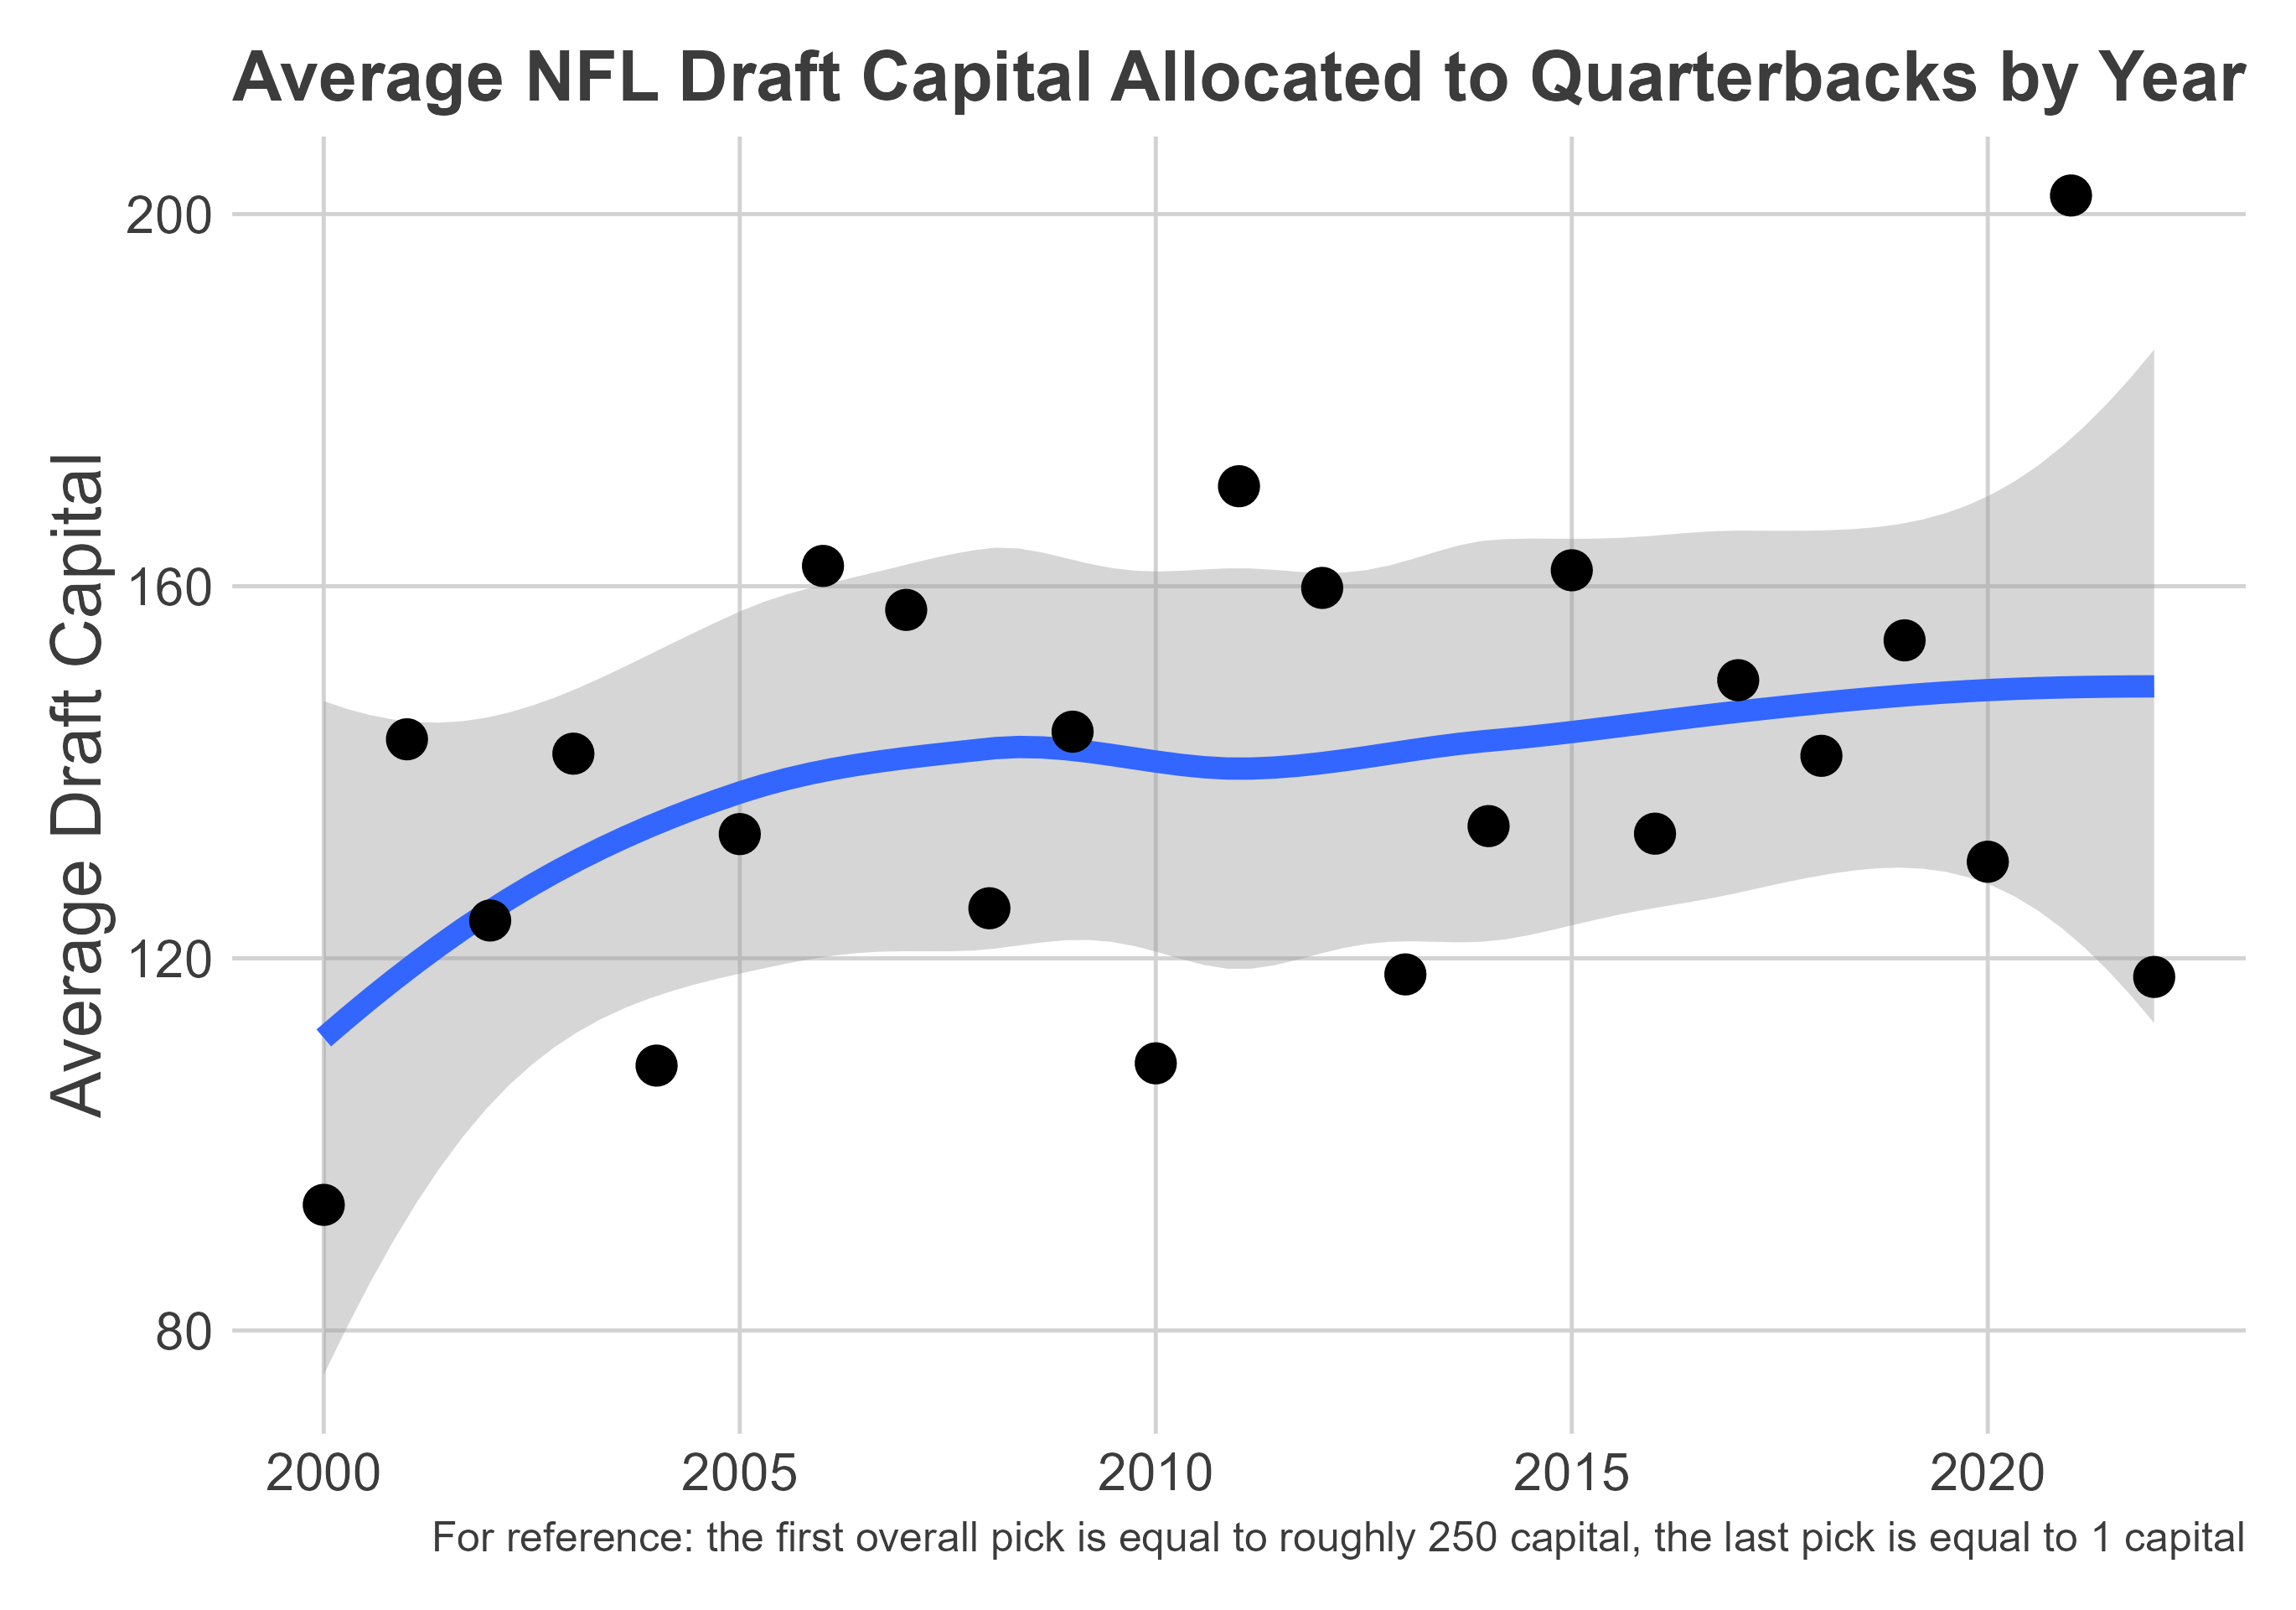
\includegraphics[width=14cm]{PS6b_Plaisance.png}
        \centering
        \\}
  \newpage
  \item Finally we look at inside linebackers, which are traditionally smaller, faster and more agile than outside linebackers. In general, inside linebackers are better in coverage while outside linebackers are better run-fitters. So as the NFL has become more of a passing league, it makes sense that teams are allocating more draft capital than ever to inside linebackers.
  
    \linebreak
    \linebreak
      \parbox{\linewidth}{
        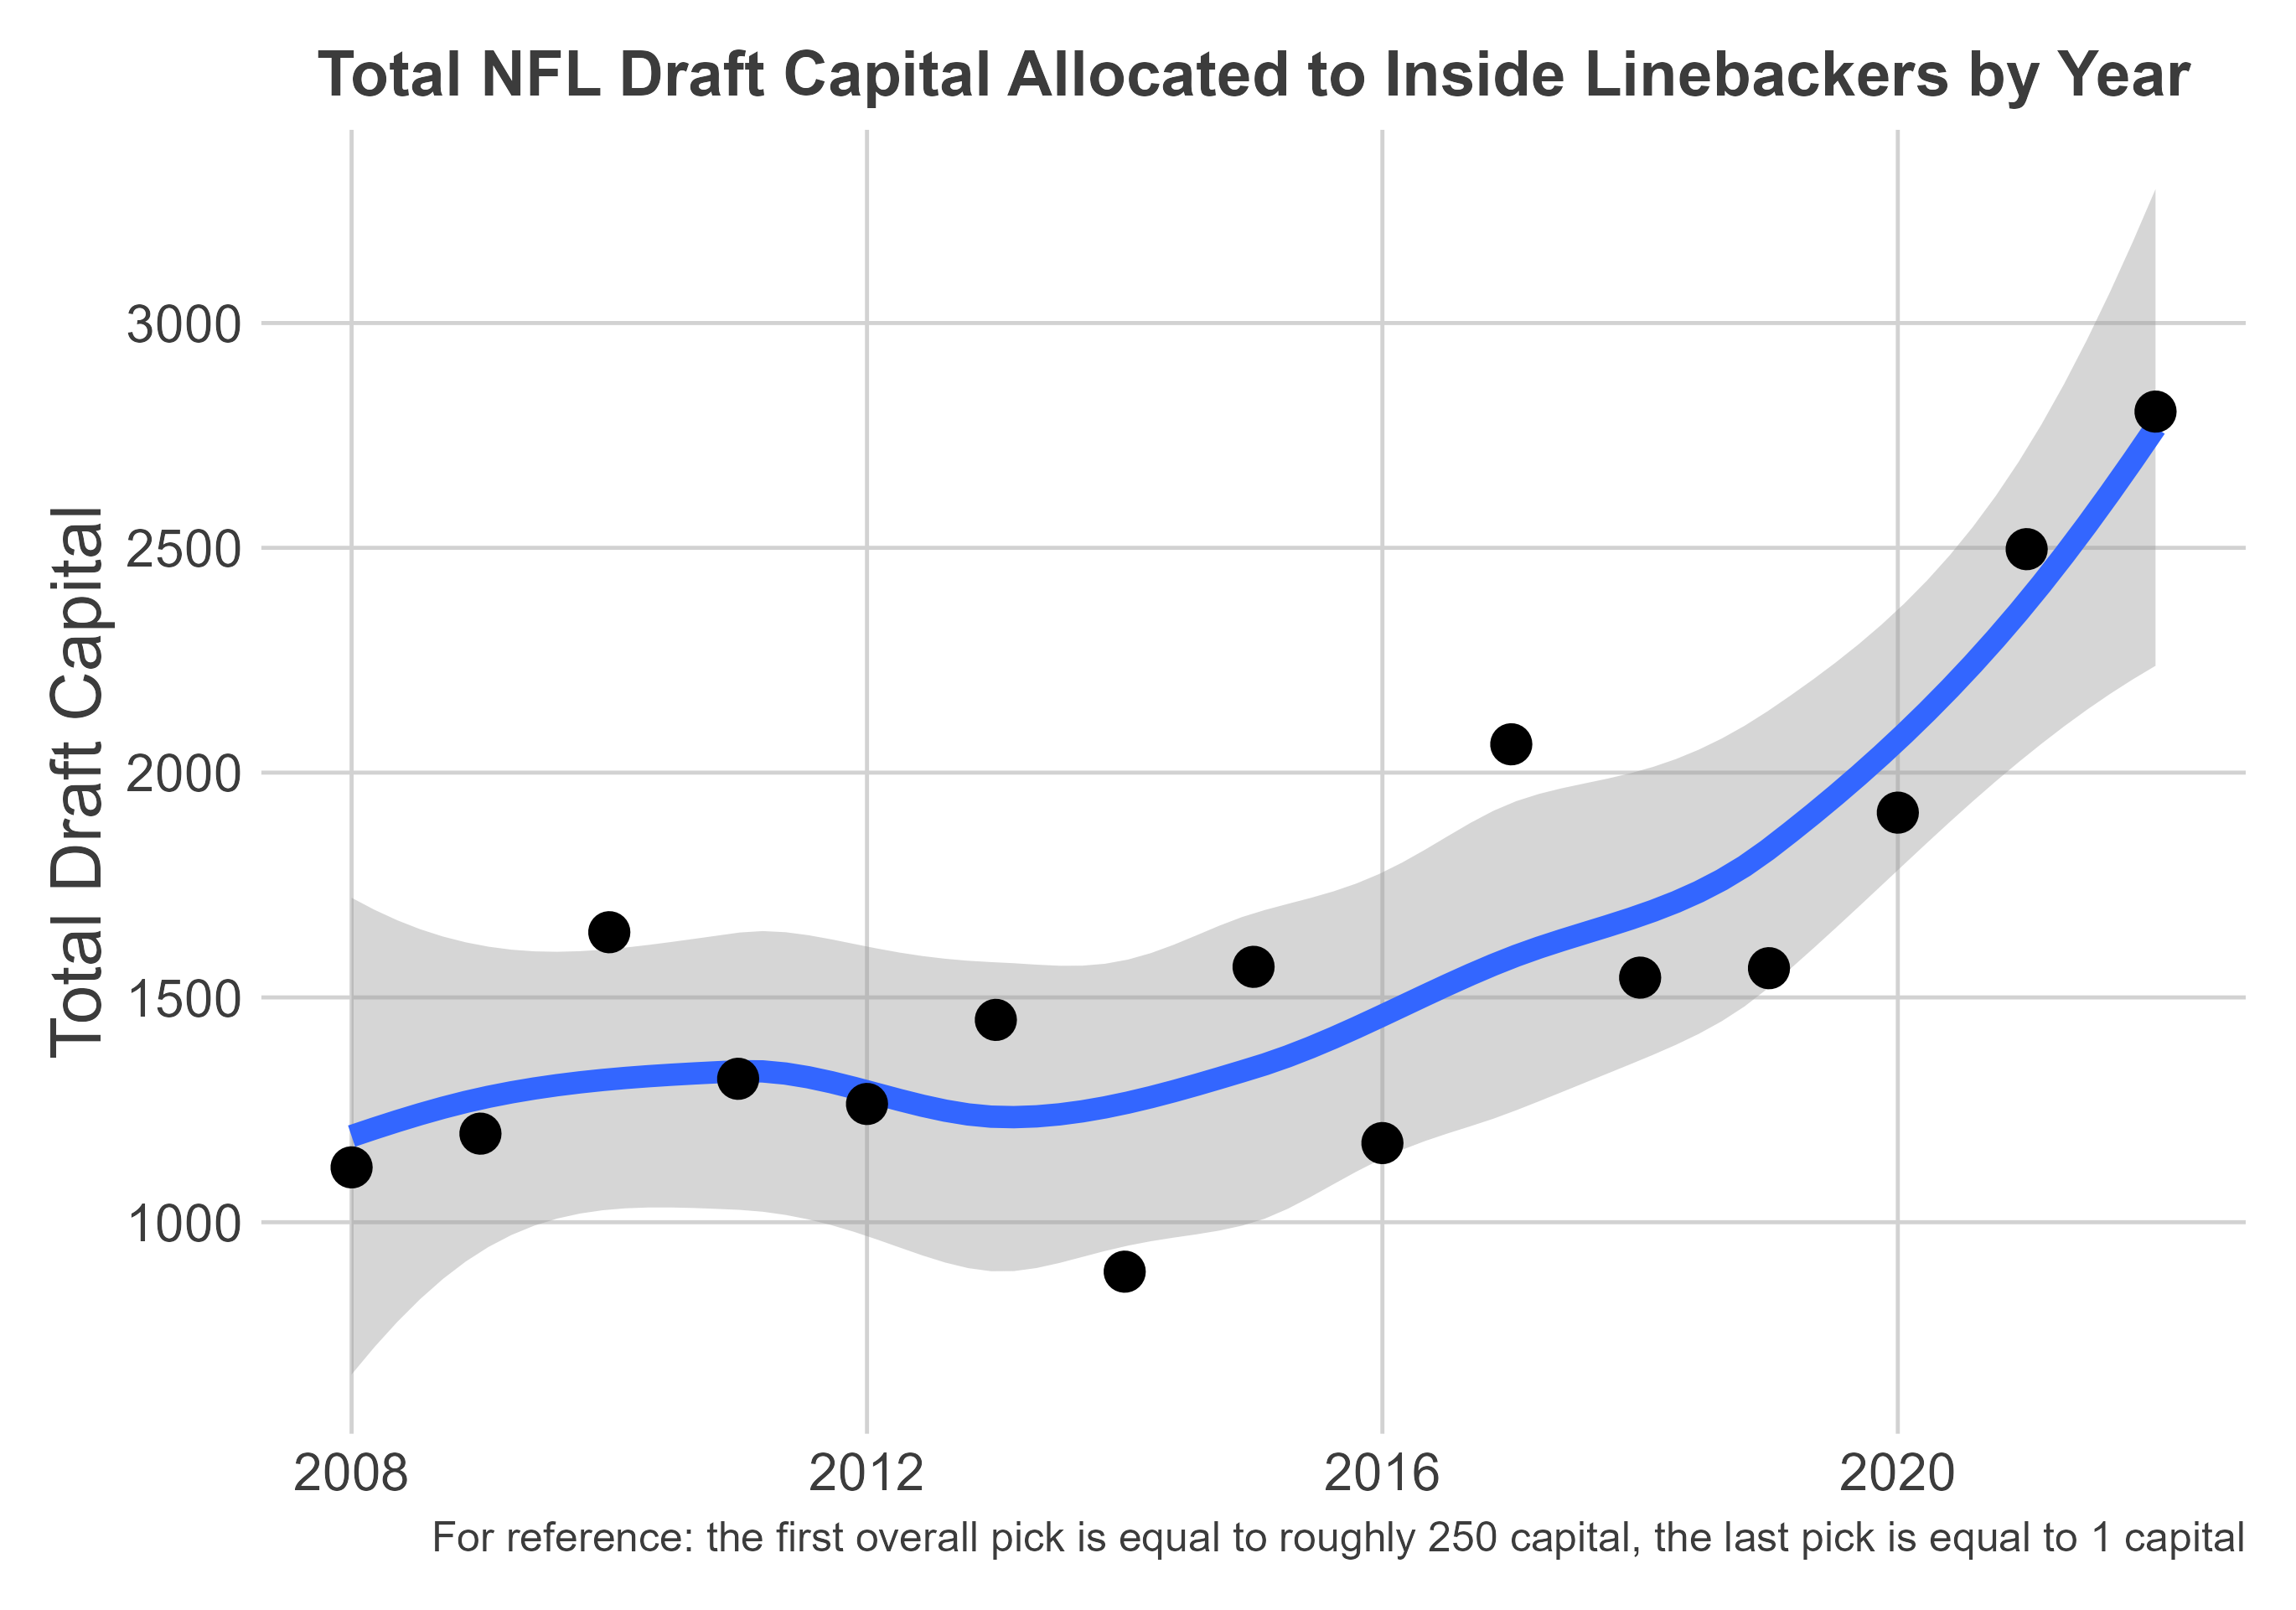
\includegraphics[width=14cm]{PS6c_Plaisance.png}
        \centering
        \\}
\end{enumerate}
\end{document}
